\subsection{Principal Minors and Inertia}

\begin{definition} \label{def:principal-and-leading-principal-minors} \hlt{Principal and Leading Principal Minors}\\
Let $n\in\mathbb{Z}_{>0}$, $\mathbb{F}\in\{\mathbb{R},\mathbb{C}\}$, and $A=[a_{ij}]\in\operatorname{Mat}(n,n,\mathbb{F})$.
\begin{enumerate}[label=(\roman*)]
\setlength{\itemsep}{0pt}
\item If $\varnothing\neq I\subseteq\{1,\ldots,n\}$, then $A[I]\defeq[a_{ij}]_{i,j\in I}$ is the \hlt{principal submatrix indexed by $I$}.\\
Its determinant $\det A[I]$ is the corresponding \hlt{principal minor}.
\item If $k\in\{1,\ldots,n\}$, then $\det A[\{1,\ldots,k\}]$ is the $k$th \hlt{leading principal minor} of $A$.
\end{enumerate}
\end{definition}

\begin{corollary} \label{cor:positive-semidefinite-principal-block-column-inclusion} \hlt{Principal Blocks and Column Inclusion}\\
Let $n\in\mathbb{Z}_{>0}$, $\mathbb{F}\in\{\mathbb{R},\mathbb{C}\}$, $k\in\{1,\ldots,n\}$, and $A\in\operatorname{Mat}(n,n,\mathbb{F})$ satisfy $A\succeq0$. Partition $A=\left(\begin{smallmatrix}A_{11}&A_{12}\\A_{12}^*&A_{22}\end{smallmatrix}\right)$ with $A_{11}\in\operatorname{Mat}(k,k,\mathbb{F})$.
\begin{enumerate}[label=(\roman*)]
\setlength{\itemsep}{0pt}
\item $A_{11}\succeq0$.
\item $\operatorname{col}(A_{12})\subseteq\operatorname{col}(A_{11})$.
\item $\operatorname{rank}(A_{12})\leq\operatorname{rank}(A_{11})$.
\item If $A\succ0$, then $A_{11}\succ0$.
\end{enumerate}
\begin{proof}
Choose $m\in\mathbb{Z}_{>0}$ and $B\in\operatorname{Mat}(m,n,\mathbb{F})$ with $A=B^*B$ by Theorem \ref{thm:positive-semidefinite-matrix-equivalences}(iv).\\
Write $B=[B_1\ B_2]$ conformally; then $A_{11}=B_1^*B_1$ and $A_{12}=B_1^*B_2$.
\begin{enumerate}[label=(\roman*)]
\setlength{\itemsep}{0pt}
\item $A_{11}\succeq0$ by Proposition \ref{prop:rectangular-gram-products-are-psd}(i).
\item $\operatorname{col}(A_{12})\subseteq\operatorname{col}(B_1^*)$ by $A_{12}=B_1^*B_2$. The identity $\operatorname{col}(B_1^*)=\operatorname{col}(B_1^*B_1)=\operatorname{col}(A_{11})$ holds by Theorem \ref{thm:gram-factor-kernel-rank-column-data}(iv).
\item $\operatorname{rank}(A_{12})=\dim\operatorname{col}(A_{12})\leq\dim\operatorname{col}(A_{11})=\operatorname{rank}(A_{11})$ by part (ii).
\item If $A\succ0$ and $\mathbf{x}\in\mathbb{F}^k\setminus\{\mathbf{0}\}$, set $\mathbf{z}\defeq\left(\begin{smallmatrix}\mathbf{x}\\\mathbf{0}\end{smallmatrix}\right)$.\\
Then $\mathbf{z}\neq\mathbf{0}$ and $\mathbf{x}^*A_{11}\mathbf{x}=\mathbf{z}^*A\mathbf{z}>0$, so $A_{11}\succ0$ by part (i) and the definition of positive definiteness.
\end{enumerate}
\hlt{Structural Commentary}: The Gram partition proves the block claims; zero padding transfers strict positivity.\\
\hlt{Key Insight}: $A_{11}=B_1^*B_1$ and $A_{12}=B_1^*B_2$ share the same left factor.
\end{proof}
\end{corollary}

Figure \ref{fig:principal-block-column-inclusion} highlights the principal and cross blocks involved in the positive-semidefinite column-inclusion result.

\begin{illustrationfigure}[H]
  \centering
  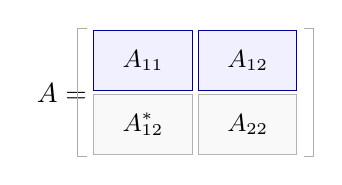
\begin{tikzpicture}[
  every node/.style={font=\small},
  block/.style={draw=gray!60, fill=gray!5, minimum width=1.25cm, minimum height=0.76cm, align=center},
  focus/.style={draw=blue!60!black, fill=blue!6}
]
  \node[block, focus] (a11) at (0,0) {$A_{11}$};
  \node[block, focus] (a12) at (1.33,0) {$A_{12}$};
  \node[block] (a21) at (0,-0.81) {$A_{12}^*$};
  \node[block] (a22) at (1.33,-0.81) {$A_{22}$};

  \node[font=\normalsize] at (-1.03,-0.41) {$A=$};
  \draw[gray!65] (-0.71,0.41) -- (-0.83,0.41) -- (-0.83,-1.22) -- (-0.71,-1.22);
  \draw[gray!65] (2.04,0.41) -- (2.16,0.41) -- (2.16,-1.22) -- (2.04,-1.22);
\end{tikzpicture}

  \caption{For $A\succeq0$, factorisation forces $\operatorname{col}(A_{12})\subseteq\operatorname{col}(A_{11})$.}
  \label{fig:principal-block-column-inclusion}
\end{illustrationfigure}

\begin{theorem} \label{thm:sylvester-positive-definite-criterion-leading-minors} \hlt{Sylvester's Criterion}\\
Let $n\in\mathbb{Z}_{>0}$, $\mathbb{F}\in\{\mathbb{R},\mathbb{C}\}$, and let $A\in\operatorname{Mat}(n,n,\mathbb{F})$ satisfy $A=A^*$. Then $A\succ0$ iff $(\forall\,k\in\{1,\ldots,n\})\,\det A[\{1,\ldots,k\}]>0$.
\begin{proof}
\begin{enumerate}[label=\roman*.]
\setlength{\itemsep}{0pt}
\item[$(\Rightarrow)$] The relation $A\succeq0$ holds by positive definiteness. Fix $k\in\{1,\ldots,n\}$ and set $A_k\defeq A[\{1,\ldots,k\}]$.\\
Then $A_k\succ0$ by Corollary \ref{cor:positive-semidefinite-principal-block-column-inclusion}(iv), so $A_k\succeq0$ by definition and $\det A_k>0$ by Proposition \ref{prop:trace-determinant-positive-semidefinite}(iv).
\item[$(\Leftarrow)$] Induct on $n$. If $n=1$, then $A=[a]$ with $a>0$, so $A\succ0$ by definition. Assume $n\geq2$ and the converse in dimension $n-1$.\\
Write $A=\left(\begin{smallmatrix}B&\mathbf{y}\\\mathbf{y}^*&a\end{smallmatrix}\right)$. Then $B=B^*$ and its leading principal minors are positive, so $B\succ0$ by the induction hypothesis and $B$ is invertible by Theorem \ref{thm:positive-definite-matrix-equivalences}(iii). Set $\delta\defeq a-\mathbf{y}^*B^{-1}\mathbf{y}$. Then $\delta=\frac{\det A}{\det B}>0$ by Proposition \ref{prop:schur-complement-determinant-formula} and leading-minor hypothesis.\\
For $\mathbf{z}=\left(\begin{smallmatrix}\mathbf{u}\\t\end{smallmatrix}\right)$, set $\mathbf{w}\defeq\mathbf{u}+B^{-1}\mathbf{y}t$. Then $\mathbf{z}^*A\mathbf{z}=\mathbf{w}^*B\mathbf{w}+\delta\abs{t}^2$ by direct expansion. Terms nonnegative by $B\succ0$, $\delta>0$.\\
For $\mathbf{z}\neq\mathbf{0}$, $t\neq0\Rightarrow\delta\abs{t}^2>0$, while $t=0\Rightarrow\mathbf{w}=\mathbf{u}\neq\mathbf{0}\Rightarrow\mathbf{w}^*B\mathbf{w}>0$. Thus $A\succ0$ by definition.
\end{enumerate}
\hlt{Structural Commentary}: Induction handles the leading block; the Schur complement supplies the final square coefficient.\\
\hlt{Key Insight}: Positive leading minors make every completed-square pivot positive.
\end{proof}
\end{theorem}

\begin{computationmethod} \label{meth:two-by-two-quadratic-form-test} \hlt{$2\times2$ Quadratic Form Test}\\
Given a real symmetric matrix $A=\left(\begin{smallmatrix}a&b\\b&c\end{smallmatrix}\right)$, set $q(x,y)\defeq ax^2+2bxy+cy^2$.\\
The output is the sign classification of $q$. Set $\Delta\defeq ac-b^2$ and proceed as follows:
\begin{enumerate}[label=(\roman*)]
\setlength{\itemsep}{0pt}
\item If $a\neq0$, complete the square as $q(x,y)=a\left(x+\frac{b}{a}y\right)^2+\frac{\Delta}{a}y^2$.
\item If $a=0$ and $c\neq0$, interchange $x$ and $y$ and repeat part (i); if $a=c=0$, inspect $q(x,y)=2bxy$ directly.
\item Conclude that $A\succ0$ iff $a>0$ and $\Delta>0$, while $-A\succ0$ iff $a<0$ and $\Delta>0$.
\item Conclude that $q$ takes both positive and negative values iff $\Delta<0$.
\item If $\Delta=0$, conclude that $A\succeq0$ iff $a,c\geq0$, while $-A\succeq0$ iff $a,c\leq0$.
\end{enumerate}
The strict classifications in part (iii) agree with Theorem \ref{thm:sylvester-positive-definite-criterion-leading-minors}.\\
The completed-square and zero-diagonal branches determine parts (iv) and (v).
\end{computationmethod}

\begin{theorem} \label{thm:real-quadratic-form-principal-axes} \hlt{Principal Axes for Real Quadratic Forms}\\
Let $n\in\mathbb{Z}_{>0}$ and let $A\in\operatorname{Mat}(n,n,\mathbb{R})$ satisfy $A=A^t$. Set $q_A(\mathbf{x})\defeq\mathbf{x}^tA\mathbf{x}$.
\begin{enumerate}[label=(\roman*)]
\setlength{\itemsep}{0pt}
\item $(\exists\,Q\in\operatorname{Mat}(n,n,\mathbb{R}))(\exists\,\lambda_1,\ldots,\lambda_n\in\mathbb{R})[Q^tQ=I_n\land A=Q\operatorname{diag}(\lambda_1,\ldots,\lambda_n)Q^t]$. Let $Q,\lambda_1,\ldots,\lambda_n$ be any choice satisfying these conditions.\\
Then $(\forall\,\mathbf{x}\in\mathbb{R}^n)\,q_A(\mathbf{x})=\sum\limits_{j=1}^{n}\lambda_j(Q^t\mathbf{x})_j^2$. Parts (ii)--(iv) are stated with respect to this choice.
\item $A\succeq0$ iff $(\forall\,j\in\{1,\ldots,n\})\,\lambda_j\geq0$.
\item $A\succ0$ iff $(\forall\,j\in\{1,\ldots,n\})\,\lambda_j>0$.
\item $q_A$ takes both positive and negative values iff $(\exists\,j,k\in\{1,\ldots,n\})[\lambda_j>0\land\lambda_k<0]$.
\end{enumerate}
\begin{proof}
\begin{enumerate}[label=(\roman*)]
\setlength{\itemsep}{0pt}
\item[$(i)$] Fix an orthogonal $Q_0$ and $\mu_1,\ldots,\mu_n\in\mathbb{R}$ with $A=Q_0\operatorname{diag}(\mu_1,\ldots,\mu_n)Q_0^t$ by Theorem \ref{thm:real-spectral-theorem}(i)$\Rightarrow$(iii).\\
Then $(\forall\,\mathbf{x}\in\mathbb{R}^n)\,q_A(\mathbf{x})=\sum\limits_{j=1}^{n}\mu_j(Q_0^t\mathbf{x})_j^2$. For parts (ii)--(iv), fix any $Q,\lambda_1,\ldots,\lambda_n$ satisfying part (i).
\item[$(ii)$] ($\Rightarrow$) $(\forall\,j\in\{1,\ldots,n\})\,\lambda_j=q_A(Q\mathbf{e}_j)\geq0$ by part (i) and $A\succeq0$.
\item[$(ii)$] ($\Leftarrow$) $(\forall\,\mathbf{x}\in\mathbb{R}^n)\,q_A(\mathbf{x})\geq0$ by part (i) and $(\forall\,j\in\{1,\ldots,n\})\,\lambda_j\geq0$. Thus $A\succeq0$ by $A=A^t$ and definition.
\item[$(iii)$] ($\Rightarrow$) $(\forall\,j\in\{1,\ldots,n\})\,\lambda_j=q_A(Q\mathbf{e}_j)>0$ by part (i) and $A\succ0$.
\item[$(iii)$] ($\Leftarrow$) If $\mathbf{x}\neq\mathbf{0}$, then $Q^t\mathbf{x}\neq\mathbf{0}$ and $q_A(\mathbf{x})>0$ by part (i) and $(\forall\,j\in\{1,\ldots,n\})\,\lambda_j>0$. Thus $A\succ0$ by $A=A^t$ and definition.
\item[$(iv)$] ($\Rightarrow$) If $\mathbf{u},\mathbf{v}\in\mathbb{R}^n$ satisfy $q_A(\mathbf{u})>0>q_A(\mathbf{v})$, then $(\exists\,j,k\in\{1,\ldots,n\})[\lambda_j>0\land\lambda_k<0]$ by part (i).
\item[$(iv)$] ($\Leftarrow$) If $j,k\in\{1,\ldots,n\}$ satisfy $\lambda_j>0>\lambda_k$, then $q_A(Q\mathbf{e}_j)=\lambda_j>0>\lambda_k=q_A(Q\mathbf{e}_k)$.
\end{enumerate}
\hlt{Structural Commentary}: Spectral coordinates diagonalise the form; coordinate vectors and the square sum classify its signs.\\
\hlt{Key Insight}: Each eigenvalue is the form value on its eigenvector.
\end{proof}
\end{theorem}

\begin{computationmethod} \label{meth:quadratic-form-principal-axes} \hlt{Quadratic Form Principal-Axes Method}\\
Given a real quadratic form $q$ in $n$ variables, the output is an orthogonal coordinate representation of $q$ and its sign classification.
\begin{enumerate}[label=(\roman*)]
\setlength{\itemsep}{0pt}
\item Write $q(\mathbf{x})=\mathbf{x}^tA\mathbf{x}$ with $A=A^t$, assigning half of each cross-term coefficient to each of the symmetric entries $a_{ij}$ and $a_{ji}$.
\item Compute an orthogonal diagonalisation $A=Q\Lambda Q^t$.
\item Set $\mathbf{y}=Q^t\mathbf{x}$ and rewrite $q(\mathbf{x})=\sum\limits_{j=1}^{n}\lambda_jy_j^2$.
\item Classify the form from the signs of the diagonal entries of $\Lambda$ by Theorem \ref{thm:real-quadratic-form-principal-axes}(ii)--(iv).
\end{enumerate}
\end{computationmethod}

Figure \ref{fig:quadratic-form-principal-axes} illustrates the orthogonal change of coordinates underlying the principal-axes method.

\begin{illustrationfigure}[H]
  \centering
  \begin{tikzpicture}[
  >=Stealth,
  scale=0.95,
  axis/.style={->, gray!65, line width=0.65pt},
  paxis/.style={->, blue!70!black, line width=0.95pt},
  curve/.style={draw=teal!70!black, line width=0.9pt},
  every node/.style={font=\small}
]
  \draw[axis] (-2.2,0) -- (2.45,0) node[right] {$x_1$};
  \draw[axis] (0,-1.65) -- (0,1.9) node[above] {$x_2$};
  \draw[curve, rotate=28] (0,0) ellipse (1.65 and 0.72);

  \draw[paxis] (0,0) -- (1.28,0.68) node[pos=0.86, above right] {$\mathbf{q}_1$};
  \draw[paxis] (0,0) -- (-0.38,0.72) node[pos=0.86, above left] {$\mathbf{q}_2$};

  \node[align=center] at (5.15,0.95) {$\mathbf{y}=Q^t\mathbf{x}$};
  \draw[->, line width=0.8pt, gray!65] (2.55,0.25) -- (3.85,0.25);

  \begin{scope}[shift={(6.15,0)}]
    \draw[axis] (-1.85,0) -- (2.0,0) node[right] {$y_1$};
    \draw[axis] (0,-1.45) -- (0,1.6) node[above] {$y_2$};
    \draw[curve] (0,0) ellipse (1.45 and 0.65);
  \end{scope}

  \node[align=center, text=teal!60!black] at (6.15,-1.65) {$\lambda_1y_1^2+\lambda_2y_2^2$};
\end{tikzpicture}

  \caption{Orthogonal coordinates reveal the principal axes of a quadratic form.}
  \label{fig:quadratic-form-principal-axes}
\end{illustrationfigure}

\begin{definition} \label{def:star-congruence-and-hermitian-inertia} \hlt{$*$-Congruence and Hermitian Inertia}\\
Let $n\in\mathbb{Z}_{>0}$ and $A,B\in\operatorname{Mat}(n,n,\mathbb{C})$.
\begin{enumerate}[label=(\roman*)]
\setlength{\itemsep}{0pt}
\item The matrices $A$ and $B$ are \hlt{$*$-congruent} iff $(\exists\,S\in\operatorname{Mat}(n,n,\mathbb{C})^\times)\,A=SBS^*$.
\item If $A=A^*$, its \hlt{inertia} is $\operatorname{in}(A)\defeq(n_+(A),n_-(A),n_0(A))$.\\
The entries count the positive, negative, and zero eigenvalues, respectively, with algebraic multiplicity.
\end{enumerate}
\end{definition}

\begin{lemma} \label{lem:positive-subspace-dimension-inertia} \hlt{Positive Subspaces and Inertia}\\
Let $n\in\mathbb{Z}_{>0}$ and let $A\in\operatorname{Mat}(n,n,\mathbb{C})$ satisfy $A=A^*$.
\begin{enumerate}[label=(\roman*)]
\setlength{\itemsep}{0pt}
\item $\max\{\dim\mathcal{U}:\mathcal{U}\leq\mathbb{C}^n\land(\forall\,\mathbf{x}\in\mathcal{U}\setminus\{\mathbf{0}\})\,\mathbf{x}^*A\mathbf{x}>0\}=n_+(A)$.
\item $\max\{\dim\mathcal{U}:\mathcal{U}\leq\mathbb{C}^n\land(\forall\,\mathbf{x}\in\mathcal{U}\setminus\{\mathbf{0}\})\,\mathbf{x}^*A\mathbf{x}<0\}=n_-(A)$.
\end{enumerate}
\begin{proof}
\begin{enumerate}[label=(\roman*)]
\setlength{\itemsep}{0pt}
\item The matrix $A$ is normal by $A=A^*$, and its eigenvalues are real by Theorem \ref{thm:self-adjoint-eigenvalues-real}.\\
Let $\mathcal{E}_+$ and $\mathcal{E}_{\leq0}$ be the orthogonal sums of its positive and nonpositive eigenspaces by Theorem \ref{thm:complex-spectral-theorem}(i)$\Rightarrow$(ii).\\
Then $\dim\mathcal{E}_+=n_+(A)$ and $\dim\mathcal{E}_{\leq0}=n-n_+(A)$.\\
The inequalities $(\forall\,\mathbf{x}\in\mathcal{E}_+\setminus\{\mathbf{0}\})\,\mathbf{x}^*A\mathbf{x}>0$ and $(\forall\,\mathbf{x}\in\mathcal{E}_{\leq0})\,\mathbf{x}^*A\mathbf{x}\leq0$ hold by the spectral decomposition.\\
If $\dim\mathcal{U}>n_+(A)$, then $\mathcal{U}\cap\mathcal{E}_{\leq0}\neq\{\mathbf{0}\}$ by Corollary \ref{cor:large-subspaces-intersect}(i), so $\mathcal{U}$ is not positive. Thus $\mathcal{E}_+$ attains the maximal dimension $n_+(A)$.
\item A subspace is negative for $A$ iff it is positive for $-A$.\\
Its maximal dimension is $n_+(-A)=n_-(A)$ by part (i) and $(-A)\mathbf{x}=\lambda\mathbf{x}\Longleftrightarrow A\mathbf{x}=-\lambda\mathbf{x}$.
\end{enumerate}
\hlt{Structural Commentary}: A spectral sign subspace attains the bound; its complementary sign range obstructs enlargement.\\
\hlt{Key Insight}: Excess dimension forces intersection with the wrong-sign spectral subspace.
\end{proof}
\end{lemma}

\begin{theorem} \label{thm:sylvester-inertia-theorem-hermitian} \hlt{Sylvester's Inertia Theorem}\\
Let $n\in\mathbb{Z}_{>0}$ and let $A,B\in\operatorname{Mat}(n,n,\mathbb{C})$ be Hermitian. Then $A$ and $B$ are $*$-congruent iff $n_+(A)=n_+(B)$ and $n_-(A)=n_-(B)$.
\begin{proof}
\begin{enumerate}[label=\roman*.]
\setlength{\itemsep}{0pt}
\item[$(\Rightarrow)$] Suppose $A=SBS^*$ with $S$ invertible. The map $S^*$ preserves subspace dimension and satisfies $(S^*\mathbf{x})^*B(S^*\mathbf{x})=\mathbf{x}^*A\mathbf{x}$.\\
Thus $n_+(A)\leq n_+(B)$ and $n_-(A)\leq n_-(B)$ by Lemma \ref{lem:positive-subspace-dimension-inertia}.\\
The reverse inequalities hold by the same lemma and $B=S^{-1}A(S^{-1})^*$, so $n_+(A)=n_+(B)$ and $n_-(A)=n_-(B)$.
\item[$(\Leftarrow)$] Set $p\defeq n_+(A)=n_+(B)$, $q\defeq n_-(A)=n_-(B)$, $r\defeq n-p-q$, and $D\defeq I_p\oplus(-I_q)\oplus0_r$.\\
Fix $M\in\{A,B\}$. The matrix $M$ is normal by $M=M^*$ and its eigenvalues are real by Theorem \ref{thm:self-adjoint-eigenvalues-real}.\\
Order them as $\lambda_1^{(M)},\ldots,\lambda_n^{(M)}$ by positive, negative, and zero sign. Set $\Lambda_M\defeq\operatorname{diag}(\lambda_1^{(M)},\ldots,\lambda_n^{(M)})$.\\
Fix a unitary $U_M$ with $M=U_M\Lambda_MU_M^*$ by Theorem \ref{thm:complex-spectral-theorem}(i)$\Rightarrow$(iii). Set $d_j^{(M)}\defeq\sqrt{\abs{\lambda_j^{(M)}}}$ for $\lambda_j^{(M)}\neq0$ and $d_j^{(M)}\defeq1$ otherwise.\\
Put $E_M\defeq\operatorname{diag}(d_1^{(M)},\ldots,d_n^{(M)})$ and $R_M\defeq U_ME_M$. Then $R_M$ is invertible, $\Lambda_M=E_MDE_M$, and $M=R_MDR_M^*$.\\
The construction defines $R_A,R_B$. For $S\defeq R_AR_B^{-1}$, $SBS^*=R_ADR_A^*=A$, so $A$ and $B$ are $*$-congruent.
\end{enumerate}
\hlt{Structural Commentary}: Sign-subspace transport proves invariance; spectral rescaling constructs the shared signed diagonal form.\\
\hlt{Key Insight}: $I_p\oplus(-I_q)\oplus0_r$ is the complete $*$-congruence invariant.
\end{proof}
\end{theorem}

Figure \ref{fig:sylvester-inertia-congruence} summarizes the $*$-congruence reduction to positive, negative, and zero coordinate directions.

\begin{illustrationfigure}[H]
  \centering
  \begin{tikzpicture}[
  >=Stealth,
  scale=0.92,
  axis/.style={->, gray!65, line width=0.65pt},
  posregion/.style={draw=blue!70!black, fill=blue!8, line width=0.9pt},
  negregion/.style={draw=red!70!black, fill=red!8, line width=0.9pt},
  zeroregion/.style={draw=gray!70, line width=0.9pt},
  lab/.style={font=\small, align=center},
  tiny/.style={font=\scriptsize, align=center}
]
  \begin{scope}
    \draw[axis] (-1.8,0) -- (1.95,0);
    \draw[axis] (0,-1.55) -- (0,1.75);
    \draw[posregion, rotate=22] (0,0) ellipse (1.45 and 0.55);
    \draw[negregion, rotate=-28] (0,0) ellipse (0.52 and 1.15);
    \draw[zeroregion] (-1.1,-1.1) -- (1.1,1.1);
    \node[lab] at (0,-2.0) {$\mathbf{x}^*A\mathbf{x}$};
  \end{scope}

  \draw[->, line width=0.9pt, gray!70] (2.35,0) -- (3.75,0)
    node[midway, above, lab] {$*$-congruence};

  \begin{scope}[shift={(5.45,0)}]
    \draw[axis] (-1.7,0) -- (1.9,0);
    \draw[axis] (0,-1.55) -- (0,1.75);
    \draw[blue!70!black, line width=1.25pt, ->] (0,0) -- (1.35,0) node[right, tiny] {$+1$};
    \draw[red!70!black, line width=1.25pt, ->] (0,0) -- (0,-1.2) node[below, tiny] {$-1$};
    \draw[gray!65, line width=1.25pt] (-1.2,1.0) -- (1.2,1.0) node[right, tiny] {$0$};
    \node[lab] at (0,-2.0) {$I_p\oplus(-I_q)\oplus0_r$};
  \end{scope}
\end{tikzpicture}

  \caption{$*$-congruence reduces a Hermitian form to signed coordinate axes.}
  \label{fig:sylvester-inertia-congruence}
\end{illustrationfigure}
